\documentclass{beamer}

\usepackage[english]{babel}
\usepackage{amsmath,amssymb}
\usepackage{graphicx}
\usepackage{listings}
\usepackage{multicol}
\usepackage{url}
\usepackage{xcolor}

% Theme (you can change this)
\usetheme{Madrid}
\usecolortheme{default}

\usepackage{tikz}
\usetikzlibrary{arrows.meta, positioning}

\title[Math 418 Project]{Synthetic Handwriting with Generative Adversarial Networks}
\author{Micah Sherry}
\institute{Math 418}
\date{}

\begin{document}

% ---------------- TITLE ----------------
\begin{frame}
\titlepage
\end{frame}

% ---------------- ABSTRACT ----------------
\begin{frame}{Abstract}
This project investigates conditional GANs (cGANs) for generating handwritten characters using the EMNIST Balanced dataset.

\vspace{0.3cm}
Two architectures are compared:
\begin{itemize}
    \item Fully connected GAN (baseline)
    \item Convolutional GAN (improved spatial learning)
\end{itemize}

\vspace{0.3cm}
A classifier-based evaluation is used to measure synthetic image quality.
\end{frame}

% ---------------- INTRODUCTION ----------------
\begin{frame}{Introduction}
Goal: generate realistic handwritten characters using GANs.

\vspace{0.3cm}
GAN structure:
\begin{itemize}
    \item Generator: creates fake images
    \item Discriminator: distinguishes real vs fake
\end{itemize}
\centering
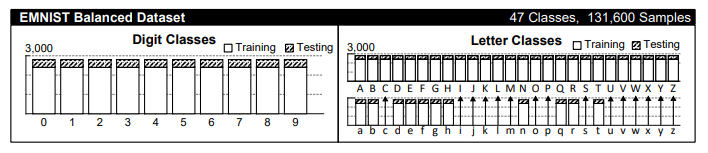
\includegraphics[width=0.85\textwidth]{images/dataset_breakdown.png}

\vspace{0.3cm}
Dataset: EMNIST Balanced (47 classes: digits + letters)


\end{frame}

% ---------------- GAN DIAGRAM ----------------
\begin{frame}{cGAN Architecture}
\begin{figure}[h]
    \centering
    \resizebox{0.95\linewidth}{!}{
    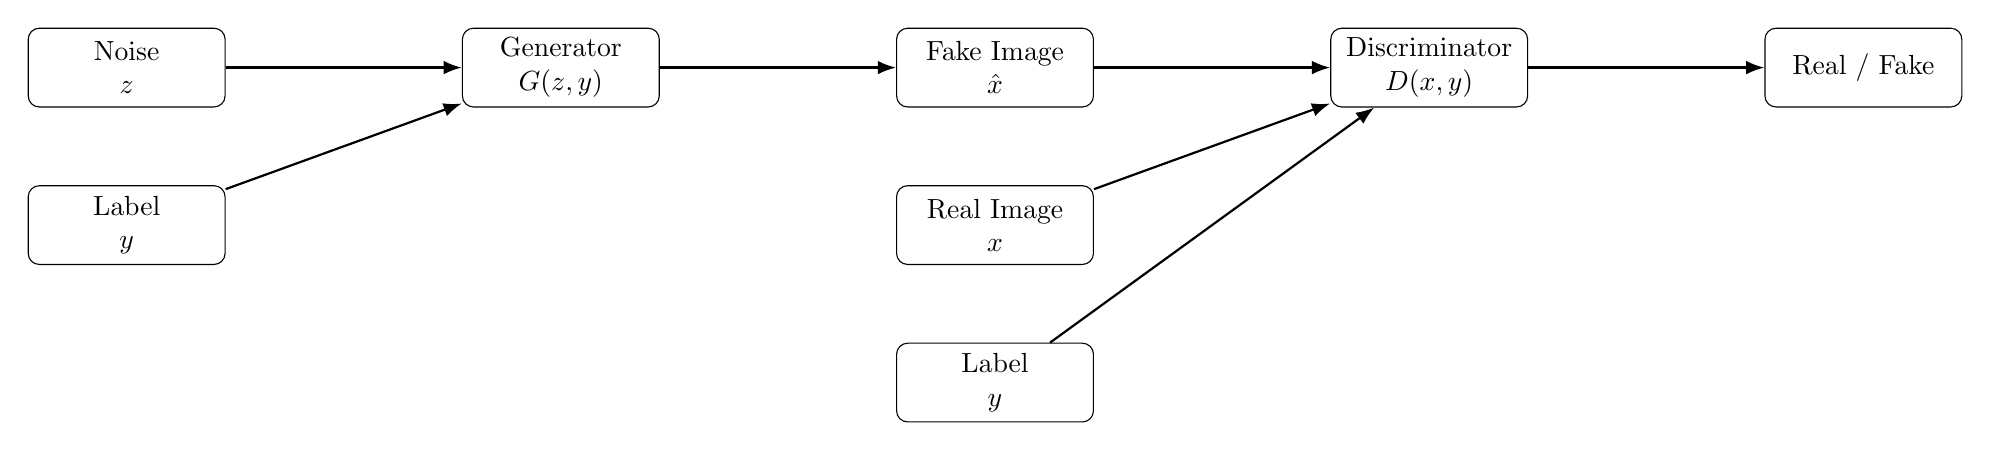
\begin{tikzpicture}[
        node distance=2cm,
        box/.style={draw, rounded corners, align=center, minimum width=2.5cm, minimum height=1cm},
        arrow/.style={-Latex, thick}
    ]
    
    % Nodes
    \node[box] (noise) {Noise \\ $z$};
    \node[box, below of=noise] (label1) {Label \\ $y$};
    
    \node[box, right=3cm of noise] (gen) {Generator \\ $G(z,y)$};
    \node[box, right=3cm of gen] (fake) {Fake Image \\ $\hat{x}$};
    
    \node[box, below of=fake] (real) {Real Image \\ $x$};
    \node[box, below of=real] (label2) {Label \\ $y$};
    
    \node[box, right=3cm of fake] (disc) {Discriminator \\ $D(x,y)$};
    \node[box, right=3cm of disc] (out) {Real / Fake};
    
    % Arrows - Generator
    \draw[arrow] (noise) -- (gen);
    \draw[arrow] (label1) -- (gen);
    \draw[arrow] (gen) -- (fake);
    
    % Arrows - Discriminator (fake path)
    \draw[arrow] (fake) -- (disc);
    
    % Arrows - Discriminator (real path)
    \draw[arrow] (real) -- (disc);
    \draw[arrow] (label2) -- (disc);
    
    % Output
    \draw[arrow] (disc) -- (out);
    
    \end{tikzpicture}
    }
    \caption{Conditional GAN (cGAN) architecture}
    
    \end{figure}

\end{frame}

% ---------------- BASELINE GAN ----------------
\begin{frame}{Traditional GAN (No Convolution)}
\textbf{Hypothesis:} Fully connected GAN will struggle with image structure.

\vspace{0.3cm}
\textbf{Training setup:}
\begin{itemize}
    \item 200 epochs
    \item Batch size: 128
    \item Noise vector: 100D
    \item Adam optimizer ($2\times10^{-4}$)
\end{itemize}

\vspace{0.3cm}
\textbf{Expected issue:} No spatial feature learning
\end{frame}

% ---------------- BASELINE RESULTS ----------------
\begin{frame}{Baseline Results}
\centering
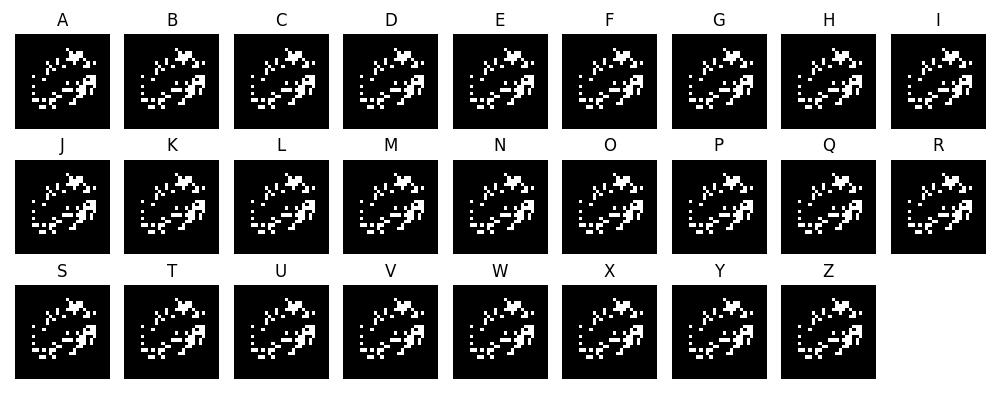
\includegraphics[width=0.75\textwidth]{images/regular/train_200.png}

\vspace{0.2cm}
Poor quality: outputs collapse and do not resemble characters
\end{frame}

% ---------------- CONV GAN ----------------
\begin{frame}{Convolutional GAN}
Why convolutional layers?
\begin{itemize}
    \item Capture edges, strokes, curves
    \item Preserve spatial structure
    \item Better for image generation
\end{itemize}

\vspace{0.3cm}
Architecture:
\begin{itemize}
    \item Generator: ConvTranspose layers
    \item Discriminator: CNN classifier
\end{itemize}
\end{frame}

% ---------------- CONV RESULTS ----------------
\begin{frame}{Conv GAN Results (Early)}
\centering
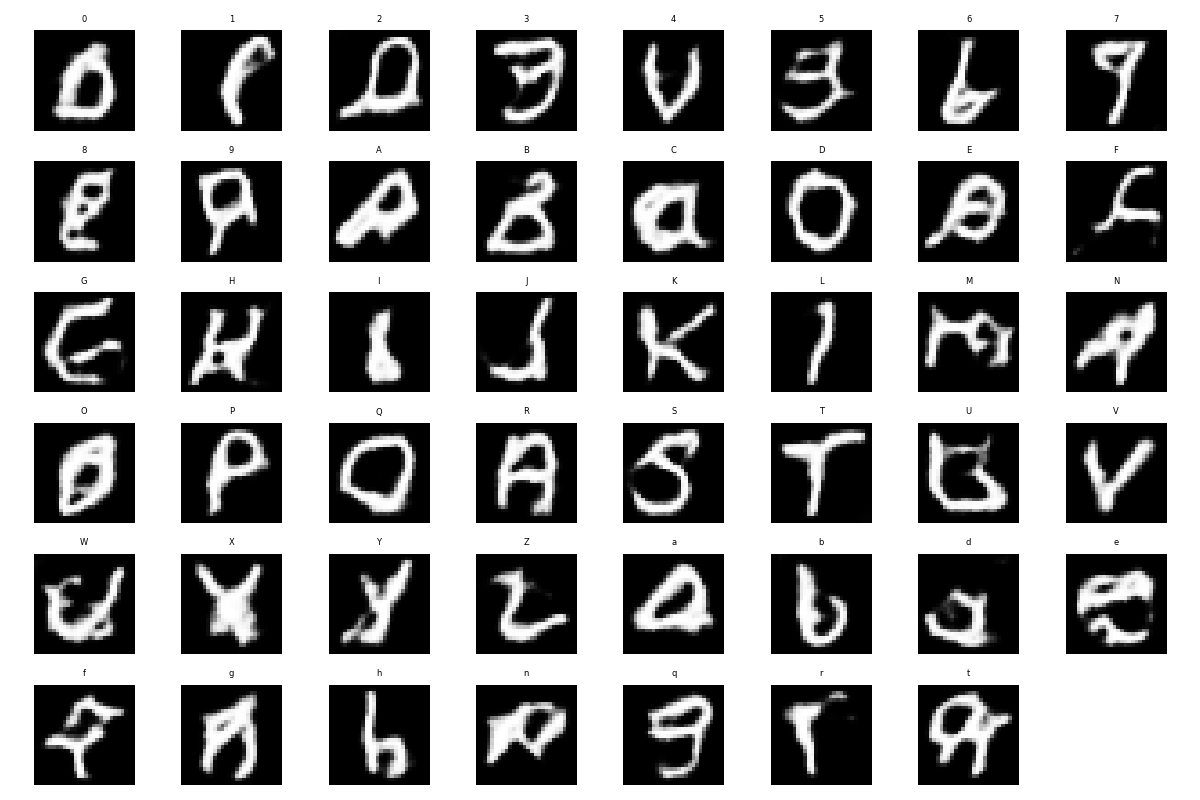
\includegraphics[width=0.75\textwidth]{images/conv/epoch_5.png}

\vspace{0.2cm}
After 5 epochs: already forming recognizable shapes
\end{frame}

\begin{frame}{Conv GAN Results (Final)}
\centering
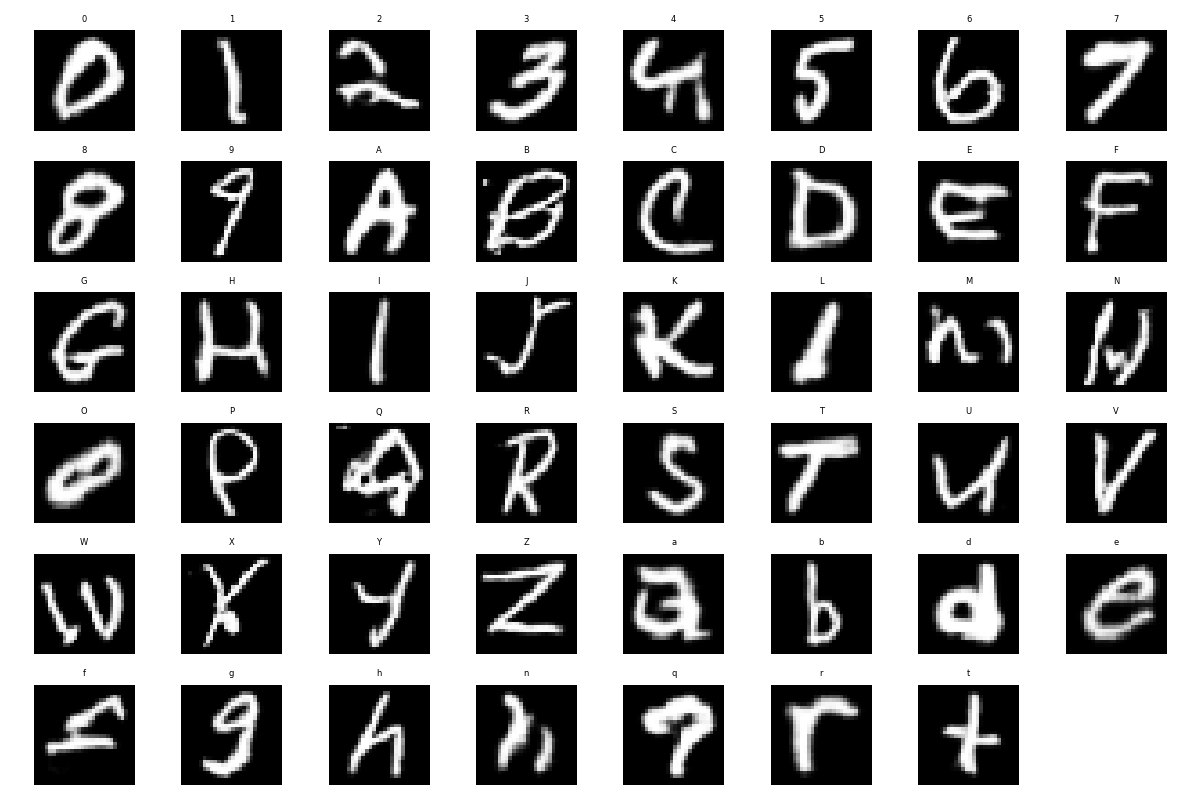
\includegraphics[width=0.75\textwidth]{images/conv/epoch_100.png}

\vspace{0.2cm}
After 100 epochs: realistic handwritten characters
\end{frame}

% ---------------- BENCHMARKING ----------------
\begin{frame}{Evaluation Method}
Image quality is subjective → use classifier-based scoring.

\vspace{0.3cm}
Pipeline:
\begin{itemize}
    \item Train classifier on real EMNIST
    \item Generate synthetic dataset
    \item Measure classification accuracy
\end{itemize}
\end{frame}

% ---------------- ACCURACY ----------------
\begin{frame}{Classification Accuracy}
\centering
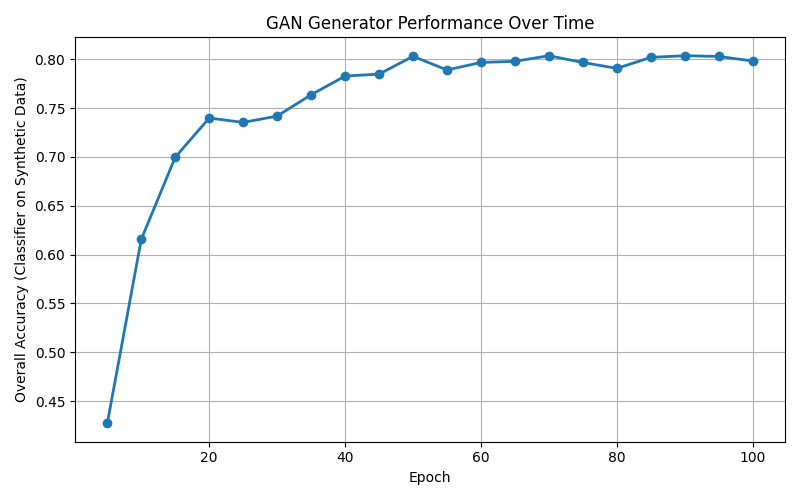
\includegraphics[width=0.8\textwidth]{images/accuracy_by_epoch.png}

\vspace{0.2cm}
Accuracy increases over training → improved generator quality
\end{frame}

% ---------------- PER CLASS ----------------
\begin{frame}{Per-Class Performance}
\centering
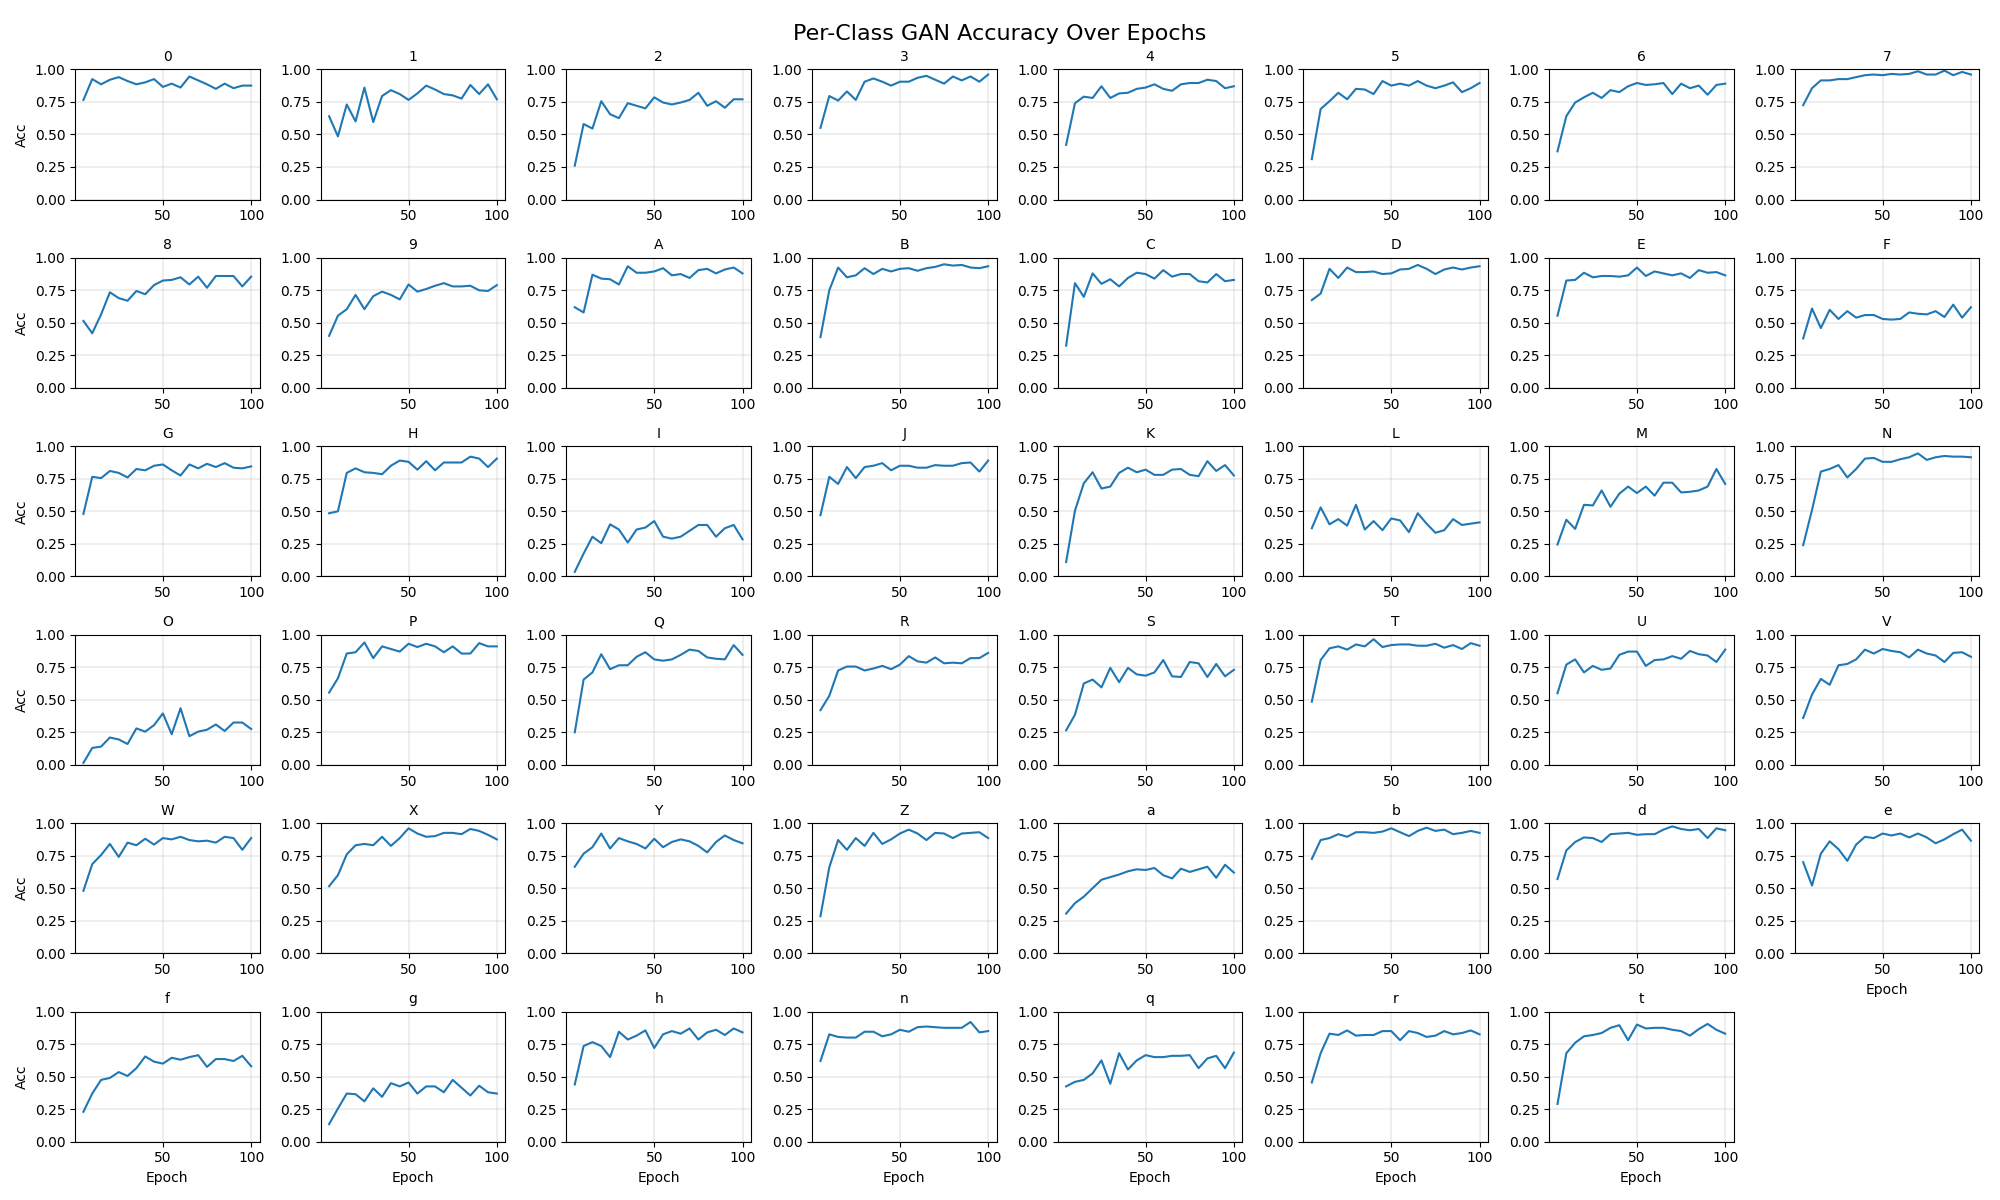
\includegraphics[width=\textwidth]{images/per_class_subplots.png}

\vspace{0.2cm}
Confusions occur between similar characters (O vs 0, g vs 9, etc.)
\end{frame}

% ---------------- PROGRESSION ----------------
\begin{frame}{Generation Progression}
\begin{itemize}
    \item Fixed noise vector across epochs
\end{itemize}
    \centering
    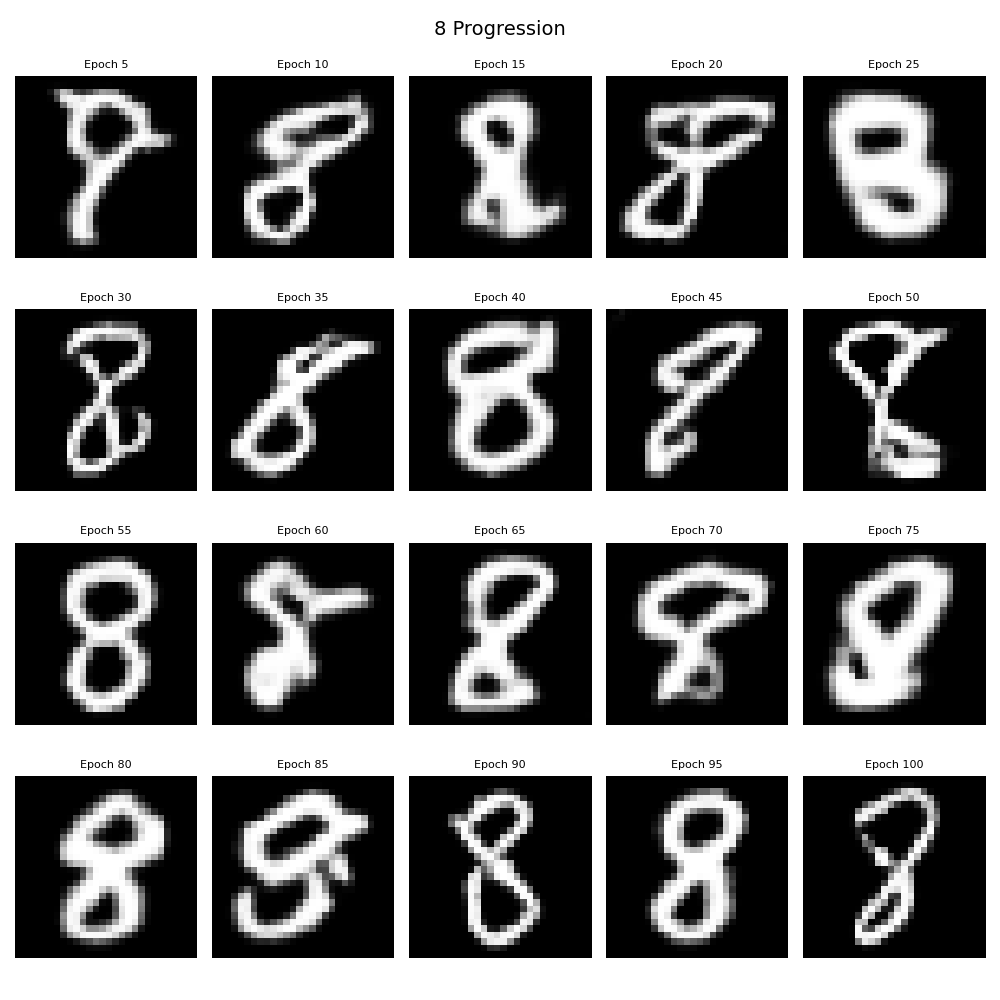
\includegraphics[width=.5\linewidth]{images/progress/label_8_progression.png}
    \end{frame}

\begin{frame}{Generation Progression}  
    \centering
    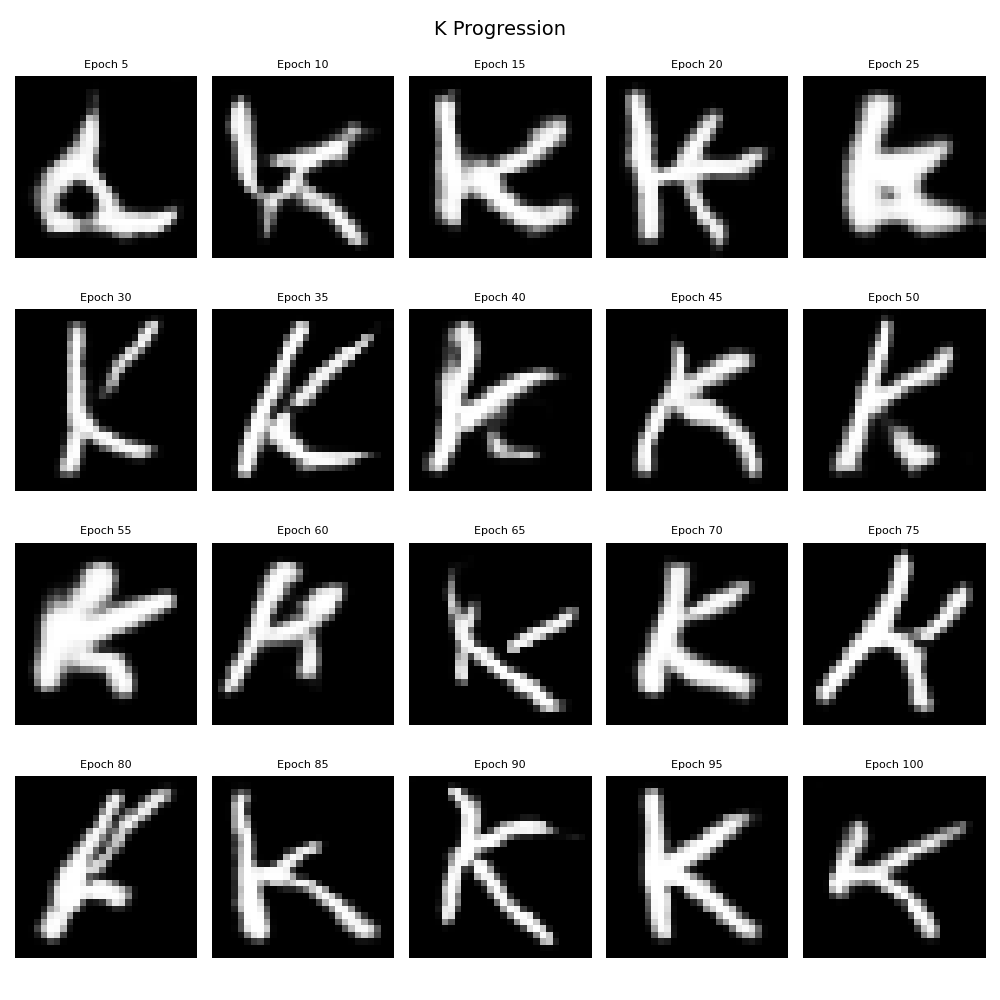
\includegraphics[width=.5\linewidth]{images/progress/label_K_progression.png}
    
\end{frame}

\begin{frame}{Generation Progression}   
    \centering
    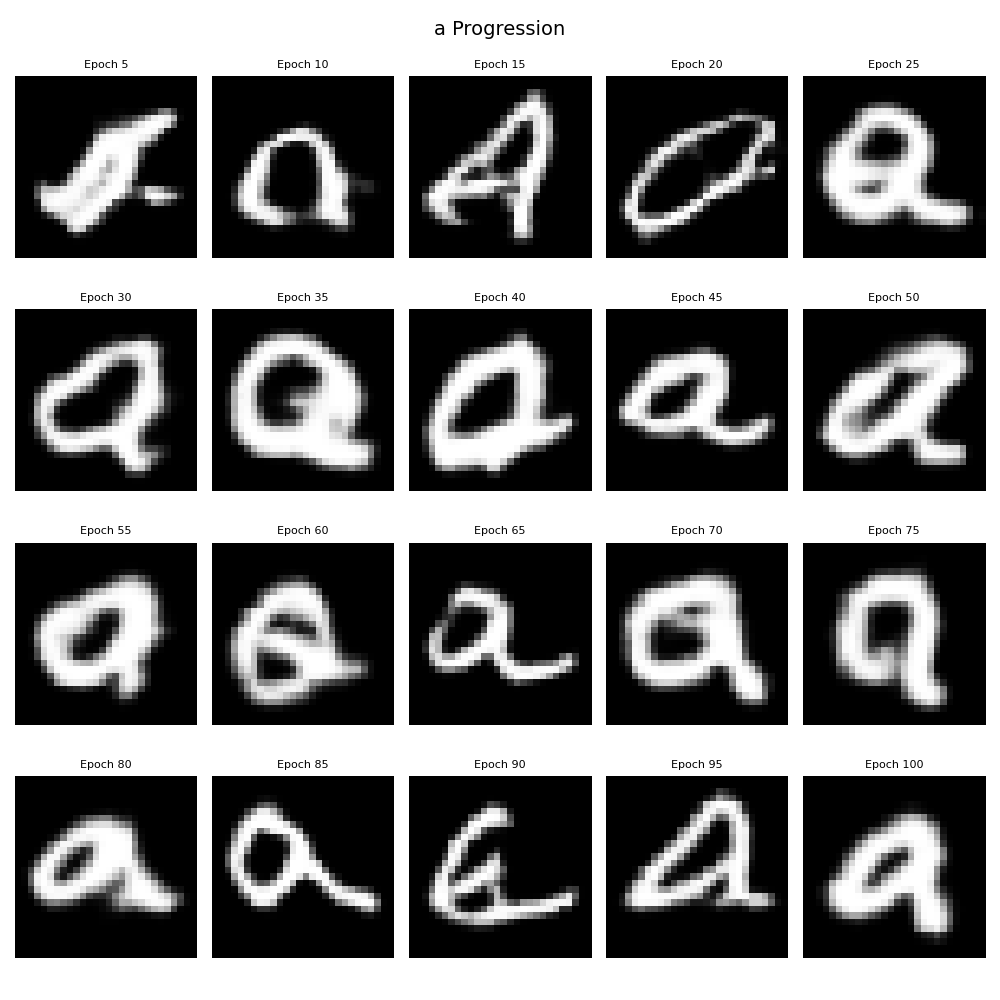
\includegraphics[width=.5\linewidth]{images/progress/label_a_progression.png}
\end{frame}

% ---------------- NOISE VARIATION ----------------
\begin{frame}{Effect of Noise Variation}
\begin{itemize}
    \item Same class, different noise vectors    
\end{itemize}
\centering
    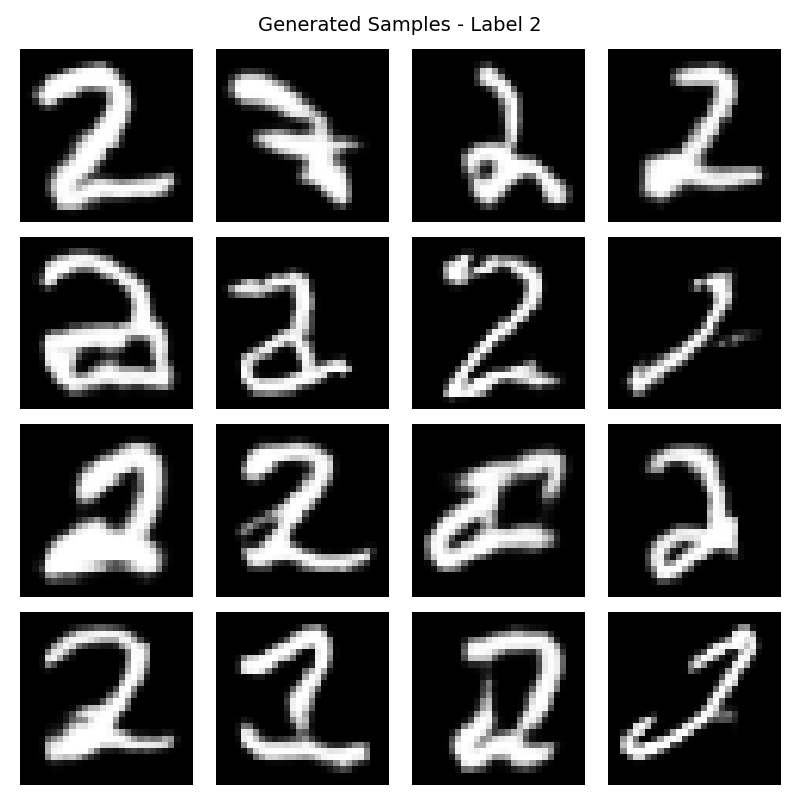
\includegraphics[width=.5\linewidth]{images/noise/noise_2.png}
\end{frame}

\begin{frame}{Effect of Noise Variation}
    \centering
    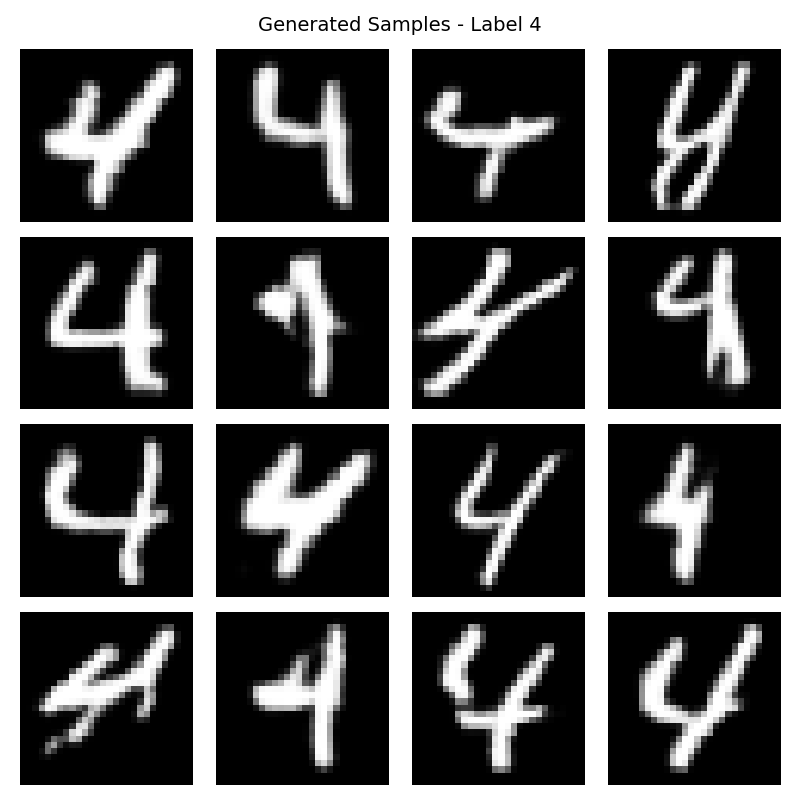
\includegraphics[width=.5\linewidth]{images/noise/noise_4.png}
\end{frame}

\begin{frame}{Effect of Noise Variation}
    \centering
    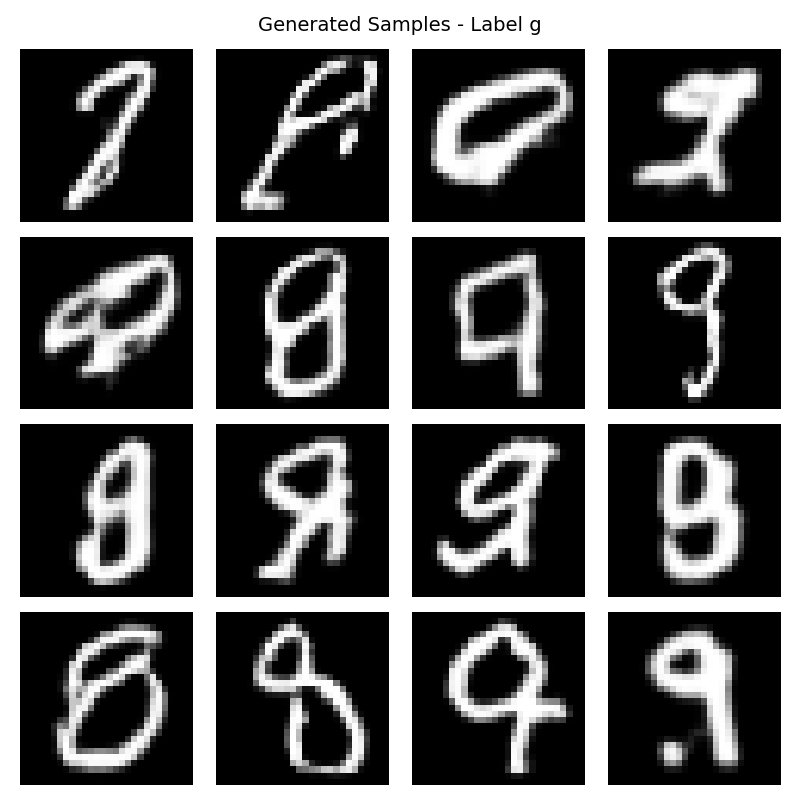
\includegraphics[width=.5\linewidth]{images/noise/noise_g.png}

\end{frame}

% ---------------- APPLICATIONS ----------------
\begin{frame}{Applications}
Synthetic handwritten text generation:

\begin{itemize}
    \item Words
    \item Digits
    \item Full sentences / quotes
\end{itemize}
\end{frame}

\begin{frame}{Generated Examples}
\centering
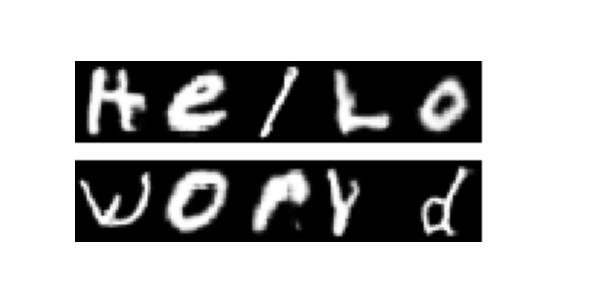
\includegraphics[width=0.85\textwidth]{images/text/Hello_world.png}

\vspace{0.2cm}
"Hello world"
\end{frame}

\begin{frame}{Generated Quote}
\centering
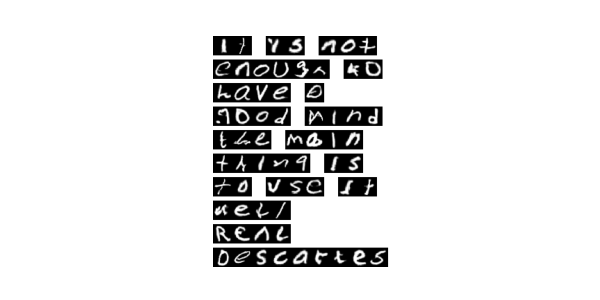
\includegraphics[width=0.85\textwidth]{images/text/It_is_not_enough_to_have_a_good_mind_the_main_thing_is_to_use_it_well____Rene_Descartes.png}
\end{frame}

% ---------------- FUTURE WORK ----------------
\begin{frame}{Further Study}
\begin{itemize}
    \item Personal handwriting style modeling
    \item Class-specific GANs
    \item Improved preprocessing
    \item Better class separation
    \item Noise-controlled style generation
\end{itemize}
\end{frame}

% ---------------- CONCLUSION ----------------
\begin{frame}{Conclusion}
\begin{itemize}
    \item Convolutional GANs dramatically outperform fully connected GANs
    \item Generated samples become realistic over training
    \item Classifier provides useful quantitative evaluation
    \item EMNIST is a strong benchmark for generative models
\end{itemize}
\end{frame}




\end{document}